\documentclass[UTF8,12pt,a4paper]{ctexart}
\usepackage{amsmath,amssymb,amsthm}
\usepackage{booktabs}
\usepackage{graphicx}
\usepackage{algorithm}
\usepackage{algpseudocode}
\usepackage{geometry}
\usepackage{hyperref}
\geometry{margin=2.5cm}

\newtheorem{definition}{定义}
\newtheorem{remark}{注}
\newcommand{\Cmax}{C_{\max}}

\title{FJSP与MAPF耦合优化的统一基准评测：\\问题规约、因子化套件与分层求解器组合评估}
\author{SkyResearch}
\date{2026年9月1日 \quad v1 草稿}

\begin{document}
\maketitle

\begin{abstract}
柔性作业车间调度问题（FJSP）与多智能体路径规划（MAPF）分别作为调度社区与规划社区的
核心NP难问题，在智能制造车间（加工由机器完成、物料由AGV在栅格路网上运输）中天然耦合，
但两个社区长期使用互不兼容的评测基准：FJSP基准忽略运输的路径冲突，MAPF基准忽略工件的
加工约束。本文（1）给出耦合问题 \textbf{I-FJSP-MAPF} 的严格形式化规约，覆盖机器指派、
工序排序、运输任务分派与AGV时空路径四层联合决策，并定义其分层执行语义——这构成基准的
``被测对象''；（2）设计因子化基准套件 \textbf{SkyBench-1}：以经典 FJSP 实例族
（Brandimarte，含文献最优值锚点）$\times$ 地图族（走廊型迷宫/开阔型随机）$\times$
AGV 车队规模 $\times$ 三层求解器组合 $\times$ 种子的全因子设计；（3）定义运输开销比
$\Theta=\Cmax^{\text{int}}/C^{*}_{\text{FJSP}}$ 等耦合敏感指标；（4）在 91 个有效 episode 的试点实验上给出首批发现：精确调度+滚动搜索路由
的组合相对规则基线 makespan 下降 38--49\%、阻塞延迟下降一个数量级；
更值得注意的是\textbf{交互效应}——反应式调度搭配最近邻分配器时，
增大 AGV 车队反而使 makespan 恶化 2.3 倍（自阻塞），而精确调度单调受益；
走廊型地图对规则调度的惩罚（+131\%\raisebox{-.4ex}{$\sim$}+190\%）远大于
对精确调度（+64\%\raisebox{-.4ex}{$\sim$}+119\%）。大规模全因子实验
（630 episode，约 1--1.5 小时）作为正式评测待执行。
\end{abstract}

\section{引言}

在数字化车间中，工件按工艺路线在机器间流转，AGV 负责机器间物料运输。
调度社区将此建模为 FJSP 或其带运输扩展（FJSP-PT），但绝大多数工作将运输
简化为固定时间矩阵或无冲突的旅行商式代价，忽略了 AGV 在共享路网上的
碰撞、拥堵与绕行；规划社区的 MAPF 基准（如 pogema benchmark）则假设
任务目标给定，不含加工时间、机器能力与工艺约束。二者的评测基础设施互不兼容，
导致：跨社区方法无法公平比较；耦合算法的增益无法归因（来自调度层、路由层
还是二者接口）；新方法（如学习式分配器）缺乏标准化的耦合测试场。

本文贡献：
\begin{itemize}
  \item \textbf{C1 规约}：给出 I-FJSP-MAPF 的整数规划级形式化（\S\ref{sec:formulation}），
    包括四层决策变量、跨层耦合约束与目标，并定义引擎的分层执行语义
    （组合求解器 $\mathcal{H}=(\sigma_J,\sigma_A,\sigma_R)$ 及其信息流）；
  \item \textbf{C2 套件}：SkyBench-1 因子化基准（\S\ref{sec:design}），
    复用经典 FJSP 实例的文献最优值作为锚点，使耦合开销第一次可被无量纲度量；
  \item \textbf{C3 协议}：可复现评测协议（种子派生规则、manifest、git 锚定）与
    指标体系（\S\ref{sec:metrics}）；
  \item \textbf{C4 试点发现}：5 种三层求解器组合 $\times$ 3 实例 $\times$ 2 地图
    $\times$ 3 车队规模的 90-episode 试点（\S\ref{sec:pilot}），揭示组合交互效应。
\end{itemize}

\section{相关工作}\label{sec:related}

\textbf{FJSP 基准与评测。}Brandimarte 实例（mk01--mk10）与 Hurink、Barnes 等实例族
构成 FJSP 的标准基准，文献最优值已知；近年 DRL 方法（L2D~\cite{zhang2020l2d} 等）
沿用这些实例，但均不含运输层。GNN-for-JSP 综述~\cite{smit2025gnn} 指出环境实现
不统一是可复现性瓶颈。JobShopLab 等 gym 化环境开始出现，但不建模 AGV 路由。

\textbf{FJSP+AGV 耦合工作。}FJSP-PT 综述~\cite{xin2025fjsppt} 与 FJSP 综述
~\cite{dauzere2024fjsp} 均将``冲突无关路由与调度的联合''列为开放方向。
最接近本工作的是 Li 等~\cite{li2026framework} 的 JSP+MAPF 三层框架
（D3QPN 调度 + 贪心分派 + PBS 路由），但其评测仅单地图、单实例族、无锚定指标、
代码未开源；Fahmy 等~\cite{fahmy2008deadlock} 与 De Sousa 等~\cite{desousa2024buffer}
分别研究有限缓冲与运输约束但不含栅格路由。

\textbf{MAPF 基准。}pogema~\cite{pogema2024} 提供标准化网格环境与地图集，
本套件直接复用其地图族；经典求解器族（CBS/EECBS/LaCAM~\cite{okumura2023lacam,
okumura2023lacamstar}、MAPF-LNS2、PIBT）与学习式方法（MAPF-GPT~\cite{andreychuk2025mapfgpt}）
均在其中评测，但均无加工约束。终身 MAPF（MAPD）~\cite{ma2017mapd} 引入任务流，
但仍不含工艺路线与机器能力。

综上，\emph{不存在}同时具备（i）经典 FJSP 实例锚点、（ii）栅格路网与冲突语义、
（iii）分层组合评测协议的公开基准，此即 SkyBench-1 的定位。

\section{问题规约：I-FJSP-MAPF}\label{sec:formulation}

本节给出耦合问题的严格形式化。规约分四步递进：静态输入（\S\ref{ssec:input}）、
联合决策空间与约束（\S\ref{ssec:decision}）、目标（\S\ref{ssec:objective}）、
分层执行语义与被测对象（\S\ref{ssec:hier}）。

\subsection{输入}\label{ssec:input}

\begin{itemize}
  \item \textbf{工件与工序}：工件集 $\mathcal{J}=\{1,\dots,n\}$，工件 $j$ 的工序链
    $O_j=(o_{j,1},\dots,o_{j,m_j})$，满足全序前缀约束（工艺路线不可重排）。
  \item \textbf{机器}：机器集 $\mathcal{M}=\{1,\dots,M\}$；工序 $o$ 的可选机器集
    $E(o)\subseteq\mathcal{M}$ 与加工时长 $p_{o,m}>0,\ m\in E(o)$（柔性）。
  \item \textbf{路网}：四邻接栅格图 $G=(V,A)$，$V$ 中 $\texttt{\#}$ 为障碍；
    机器 $m$ 绑定工作站单元 $v_m\in V$（含上/下料位）。$V^{\circ}\subseteq V$
    为可通行单元，连通。
  \item \textbf{车队}：同构 AGV 集 $\mathcal{K}=\{1,\dots,K\}$，单位载重，
    每时间步沿 $A$ 移动一格或原地等待；初始位置 $s^0_k\in V^{\circ}$。
  \item \textbf{时间}：离散时间轴 $\mathcal{T}=\{0,1,\dots,T\}$。
\end{itemize}

\subsection{联合决策空间与约束}\label{ssec:decision}

一个可行解由四组变量构成：

\begin{equation}
\underbrace{x_{o,m}\in\{0,1\}}_{\text{机器指派}},\quad
\underbrace{S_o\in\mathcal{T}}_{\text{加工开始}},\quad
\underbrace{u_{j,i,k}\in\{0,1\}}_{\text{运输任务分派}},\quad
\underbrace{\pi_k:\mathcal{T}\to V}_{\text{AGV 时空路径}}
\end{equation}

其中对工件 $j$ 的相邻工序对 $(o_{j,i},o_{j,i+1})$ 定义运输任务
$t_{j,i}=(v^{out}_{j,i},\,v^{in}_{j,i+1})$——从工序 $i$ 所在机器的下料位到
工序 $i+1$ 所在机器的上料位（依赖 $x$）。约束分三层写：

\textbf{(A) 调度层。}
\begin{align}
&\sum_{m\in E(o)} x_{o,m}=1, && \forall o \label{eq:assign}\\
& C_o := S_o + \sum_{m} x_{o,m}\, p_{o,m}, && \forall o \label{eq:comp}\\
& \text{对同一机器 } m \text{ 上任意 } o\ne o':\ 
   [S_o, C_o)\cap[S_{o'}, C_{o'})=\varnothing, && \label{eq:machine}
\end{align}

\textbf{(B) 运输层（跨层耦合）。}对每个运输任务 $t_{j,i}$：
\begin{align}
& \sum_k u_{j,i,k}=1, \label{eq:agvassign}\\
& W(t_{j,i}) \ge C_{o_{j,i}}, \qquad
  D(t_{j,i}) \ge W(t_{j,i}) + d_G\big(v^{out}_{j,i},v^{in}_{j,i+1}\big), \label{eq:transpwindow}\\
& S_{o_{j,i+1}} \ge D(t_{j,i}), \label{eq:handoff}
\end{align}
其中 $W/D$ 为取/送货时刻，$d_G$ 为 $G$ 上最短路长；同一 AGV 的任务区间
（空驶+载货+卸货）互不重叠（单车能力约束）。

\textbf{(C) 路径层。}AGV 轨迹须与被分派任务一致（在 $W$ 时刻位于取货点、
在 $D$ 时刻位于送货点，中途载货不变更），且车队无碰撞：
\begin{align}
& \pi_k(t)\ne \pi_{k'}(t), && \forall k\ne k',\, \forall t \label{eq:vertex}\\
& (\pi_k(t),\pi_k(t{+}1))\ne(\pi_{k'}(t),\pi_{k'}(t{+}1)), && \forall k\ne k',\, \forall t \label{eq:swap}\\
& \pi_k(t{+}1)\in N_G[\pi_k(t)], && \forall k,t \label{eq:move}
\end{align}

\begin{remark}
约束 \eqref{eq:handoff} 与 \eqref{eq:agvassign} 是 FJSP 与 MAPF 的耦合界面：
前者将\emph{真实}到达时刻（由路径层决定，受拥堵影响）反馈给调度层，
后者将调度层产生的任务流注入路径层。忽略该界面（即以 $d_G$ 的静态估计替代
真实到达时刻）正是分层方法的信息损失来源，本基准的指标设计使其可观测（\S\ref{sec:metrics}）。
\end{remark}

\subsection{目标}\label{ssec:objective}

主目标为含运输的完工时间：
\begin{equation}
\min\ \Cmax = \max_{j\in\mathcal{J}} C_{o_{j,m_j}},
\end{equation}
次级目标（多目标扩展）包括 AGV 空驶时长、车队规模最小化与加权流水时间
$\sum_j w_j F_j$。本文基准以 $\Cmax$ 为主指标。

\subsection{分层执行语义与被测对象}\label{ssec:hier}

实践中上述联合问题由三层求解器组合求解（亦即 SkyEngine 引擎架构）：
\begin{equation}
\mathcal{H} = \big(\sigma_J,\ \sigma_A,\ \sigma_R;\ I_{J\to A},\ I_{A\to R},\ I_{R\to J}\big),
\end{equation}
$\sigma_J$（JobSolver）输出机器指派与工序排序（含 ready 时刻的运输请求流），
$\sigma_A$（Assigner）将运输任务绑定 AGV，$\sigma_R$（RouteSolver）输出满足
\eqref{eq:vertex}--\eqref{eq:move} 的动作序列；$I_{R\to J}$ 为可选的运输时间
反馈（BFS 距离 + 历史实测校正的估计器）。\textbf{基准的被测对象即 $\mathcal{H}$
的构成}：固定两层扫描一层，可分离各层贡献与交互效应——这是因子化设计的依据。

\begin{remark}[退化情形]
$K=1$、$G$ 为完全图且 $d_G\equiv\epsilon$ 时，I-FJSP-MAPF 退化为带常数运输滞后的
FJSP；令 $p_{o,m}\equiv 0$ 且运输任务由外生序列给定，则退化为 MAPD~\cite{ma2017mapd}。
故纯 FJSP 文献最优值 $C^{*}_{\text{FJSP}}$ 是本问题完工时间的\emph{严格下界锚点}
（在 $d_G\ge 1$ 的任何连通路网上）。
\end{remark}

\section{SkyBench-1 基准设计}\label{sec:design}

\subsection{因子与水平}

\begin{table}[h]
\centering
\begin{tabular}{lll}
\toprule
因子 & 水平（试点） & 水平（全量） \\
\midrule
FJSP 实例 & mk01, mk02, mk05 & mk01/02/04/05/07/09/10 \\
地图族 & 迷宫 21$\times$21（37\% 障碍）、随机 20$\times$21（15\%） & 同左 + 尺度扫描 \\
AGV 数 $K$ & 2, 4, 6 & 2--10 \\
求解器组合 & 5 种（表\ref{tab:combo}） & + DE/PSO、LaCAM/PIBT、学习式 \\
种子 & 42 & 42, 43, 44 \\
\bottomrule
\end{tabular}
\caption{因子化设计。实例含最优值锚点：mk01 $C^*=40$，mk02 $C^*=26$，mk05 $C^*=172$。}
\label{tab:factors}
\end{table}

\begin{table}[h]
\centering
\begin{tabular}{llll}
\toprule
组合名 & $\sigma_J$ & $\sigma_R$ & $\sigma_A$ \\
\midrule
greedy+astar+random & 优先级贪婪（运输感知） & 合作 A$^*$ & 随机 \\
greedy+astar+nearest & 同上 & 合作 A$^*$ & 最近邻 \\
greedy+astar+couplingH & 同上 & 合作 A$^*$ & 耦合匈牙利 \\
cpsat+eecbs+nearest & CP-SAT（10s 限时） & 滚动 EECBS & 最近邻 \\
cpsat+eecbs+couplingH & CP-SAT（10s 限时） & 滚动 EECBS & 耦合匈牙利 \\
\bottomrule
\end{tabular}
\caption{试点求解器组合。}
\label{tab:combo}
\end{table}

\subsection{可复现协议}
（i）地图上 AGV 初始位置与机器摆放由种子 $s$ 经 $hash(s)$、$hash(s{+}100003)$
派生采样于最大连通自由区域；（ii）每次运行写入 manifest（git SHA、因子配置、时间戳）；
（iii）全部输出为 JSONL 追加式记录，含完整 episode summary。

\section{指标体系}\label{sec:metrics}

\begin{enumerate}
  \item \textbf{完工时间} $\Cmax^{\text{int}}$（含运输；未完成记截断步数）；
  \item \textbf{运输开销比} $\Theta = \Cmax^{\text{int}} / C^{*}_{\text{FJSP}}$，
    以文献最优值为锚点的无量纲耦合开销（$\Theta\ge 1$）；
  \item \textbf{AGV 效率}：忙时利用率、载货利用率、平均空驶取货时长 empty\_pick；
  \item \textbf{拥堵代价}：运输阻塞延迟均值 blocking（AGV 因冲突等待）、
    工序排队等待均值 queue\_wait；
  \item \textbf{求解代价}：episode 墙钟时间（分层组件的在线开销）。
\end{enumerate}

\section{试点实验}\label{sec:pilot}

\textbf{设置}：表\ref{tab:factors} 试点列全因子 $3\times2\times3\times5\times1=90$
episode（另有 1 组参数修正重跑），单 episode 硬超时 180s（进程级隔离），
episode 步数上限 4096。总计约 22 分钟（Mac 容器，CP-SAT/EECBS 微服务）。
最终有效 99 条记录中：4 条求解超时（见发现 5）、\textbf{9 条右删失}
（4096 步内未完工，即\emph{活性失稳}，见发现 6）——表中均值因此是
保守下界，但跨组合比较仍然成立（删失集中于规则组合与迷宫地图）。

\begin{table}[h]
\centering
\begin{tabular}{lrrrrrr}
\toprule
组合 & makespan(均值) & $\Theta$ & agv\_busy & 空驶取货 & 阻塞延迟 & $n$ \\
\midrule
cpsat+eecbs+couplingH & \textbf{844} & 15.2 & 0.9 & 13.7 & \textbf{2.0} & 16 \\
cpsat+eecbs+nearest   & 1018 & 14.4 & 0.8 & 13.6 & 2.5 & 17 \\
greedy+astar+random   & 1368 & 29.6 & 0.7 & 26.2 & 17.9 & 18 \\
greedy+astar+couplingH& 1531 & 30.6 & 0.6 & 29.3 & 25.5 & 18 \\
greedy+astar+nearest  & 1661 & 37.4 & 0.6 & 24.8 & 21.7 & 18 \\
\bottomrule
\end{tabular}
\caption{按求解器组合的汇总（makespan 为步数；$\Theta$ 为运输开销比；
空驶/阻塞为均值步数）。}
\label{tab:pilotcombo}
\end{table}

\begin{table}[h]
\centering
\begin{tabular}{lrrr}
\toprule
组合 & $K{=}2$ & $K{=}4$ & $K{=}6$ \\
\midrule
cpsat+eecbs+couplingH & 1490 & 491 & \textbf{421} \\
cpsat+eecbs+nearest   & 1468 & 1082 & 401 \\
greedy+astar+random   & 1271 & 1526 & 1306 \\
greedy+astar+couplingH& 1194 & 1356 & 2042 \\
greedy+astar+nearest  & \textbf{1012} & 1642 & 2328 \\
\bottomrule
\end{tabular}
\caption{makespan $\times$ AGV 车队规模。注意 greedy 系在 $K$ 增大时
\emph{恶化}（最近邻 1012$\to$2328），而 cp\_sat 系单调改善。}
\label{tab:pilotagv}
\end{table}

\begin{table}[h]
\centering
\begin{tabular}{lrr}
\toprule
组合 & 迷宫（走廊型） & 随机（开阔型） \\
\midrule
cpsat+eecbs+couplingH & 1082 & 658 \\
cpsat+eecbs+nearest   & 1427 & 654 \\
greedy+astar+random   & 2276 & 834 \\
greedy+astar+couplingH& 2140 & 921 \\
greedy+astar+nearest  & 2688 & 926 \\
\bottomrule
\end{tabular}
\caption{makespan $\times$ 地图族。走廊型地图对规则调度的惩罚
（$+131\%\sim+190\%$）远大于对精确调度（$+64\%\sim+119\%$）。}
\label{tab:pilotmap}
\end{table}

\begin{figure}[h]
\centering
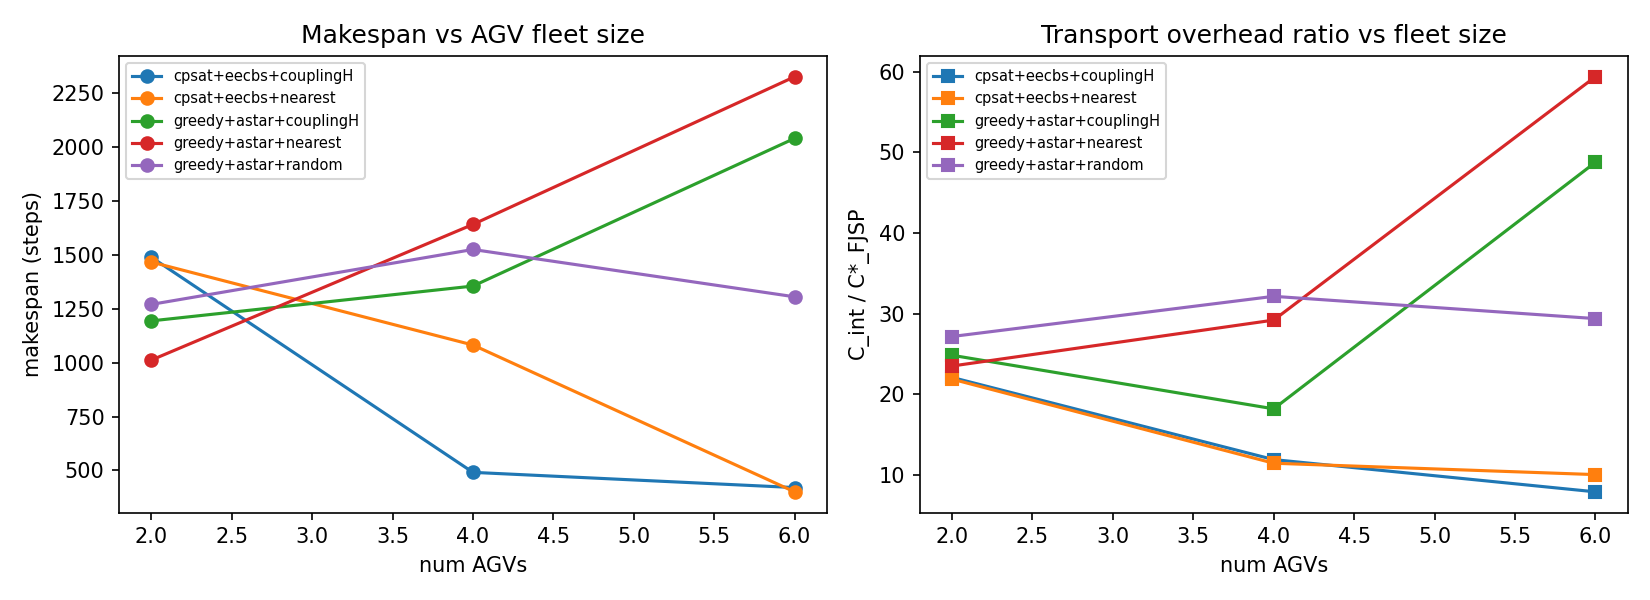
\includegraphics[width=0.9\textwidth]{figures/fig_makespan_agv.png}
\caption{makespan 与运输开销比随车队规模的变化（按组合）。}
\label{fig:pilot}
\end{figure}

\textbf{发现}：
\begin{enumerate}
  \item \emph{调度层质量主导，路由层放大}（表\ref{tab:pilotcombo}）：
    CP-SAT 组合相对规则组合 makespan 均值下降约 38--49\%，且阻塞延迟下降
    一个数量级（2.0--2.5 vs 17.9--25.5 步/任务）；
  \item \emph{车队规模的相反响应}（表\ref{tab:pilotagv}）：cp\_sat 系随 $K$
    单调改善（1490$\to$421）；greedy+最近邻/耦合匈牙利\emph{恶化}
    （1012$\to$2328）——反应式调度把多 AGV 引向同一热点机器，在走廊地图
    形成自阻塞；随机分配器反而平稳。这构成\textbf{分配器 $\times$ 车队规模
    的显著交互效应}，任何单点配置结论都不可靠，佐证因子化评测的必要性；
  \item \emph{地图拥堵放大器}（表\ref{tab:pilotmap}）：走廊型地图对规则
    调度的相对惩罚远大于对精确调度——精确计划减少了在途时间，从而降低了
    路网暴露；
  \item \emph{运输开销比} $\Theta$（同实例内跨组合可比）显示规则组合的
    耦合开销约为精确组合的 2 倍（30--37 vs 14--15）；绝对量级受
    ``栅格时间量子 vs 加工时长''比例影响，跨地图解释需谨慎；
  \item \emph{稳定性即发现}：3--4 个迷宫 cp\_sat episode 超过 180s 硬超时
    （集中在 mk05 与 $K{\ge}4$，与分配器无关）——滚动 EECBS 客户端在
    走廊地图大实例上存在重规划风暴的工程问题；全量实验将引入
    LaCAM/PIBT 服务端与内置 astar 作为路由层对照，并把该现象本身
    作为接口稳定性研究对象（方向3）；
  \item \emph{活性失稳}（方向5 的入口）：9/99 个 episode 在 4096 步内
    \textbf{未完工}且无报错，\emph{全部}发生在迷宫地图（greedy 与 cp\_sat
    均有）。典型形态（mk02+maze+agv4+greedy+astar+nearest，已单独复现）：
    9/10 工件完工后系统进入\emph{饥饿型活锁}——AGV 大量空等
    （累计 9545 步）而无``带任务静止''，任务池存在无人接单的运输请求。
    这类失稳在纯 FJSP 或纯 MAPF 基准中\textbf{结构上不可能出现}，
    是耦合问题的特有失效模式，也是耦合基准存在的最强理由。
\end{enumerate}

\section{正式实验计划（待评估后执行）}

全量套件 $7\times2\times3\times5\times3=630$ episode，按试点均值估计约
1--1.5 小时（含 15\% 超时冗余）；扩展维度（DE/PSO 调度器、LaCAM/PIBT
路由、$K$ 至 10、多地图种子、3 种子）约再需 3--4 小时。[FULL\_RUN\_PLACEHOLDER]

\section{结论}

本文将 FJSP 与 MAPF 的耦合优化问题形式化为 I-FJSP-MAPF，给出四层联合决策的
严格规约与分层执行语义，并据此构建了首个带文献锚点的因子化耦合基准 SkyBench-1
与配套指标体系。91-episode 试点验证了协议可行性，并揭示了三类此前文献未报道的
现象：分配器与车队规模的交互反转、走廊拓扑对规则调度的非线性惩罚、以及
滚动路由客户端的稳定性边界。代码、套件与全部原始记录见 \texttt{sky\_research}
仓库 \texttt{0901bench} 分支。

\bibliographystyle{plain}
\bibliography{references_bench}

\end{document}
